\section{Listen}

Eine \begriff{Liste} ist eine lineare Anordnung von Objekten des selben Typs. Eine Liste wird als verzeigerte Struktur (oder als eindimensionales Feld - wird hier aber nicht behandelt) implementiert. Eine solche Liste hat 3 Attribute:
\begin{itemize}
	\item linear vs. zyklisch
	\item einfach verkettet vs. doppelt verkettet
	\item endogen vs. exogen
\end{itemize}

\begin{center}
	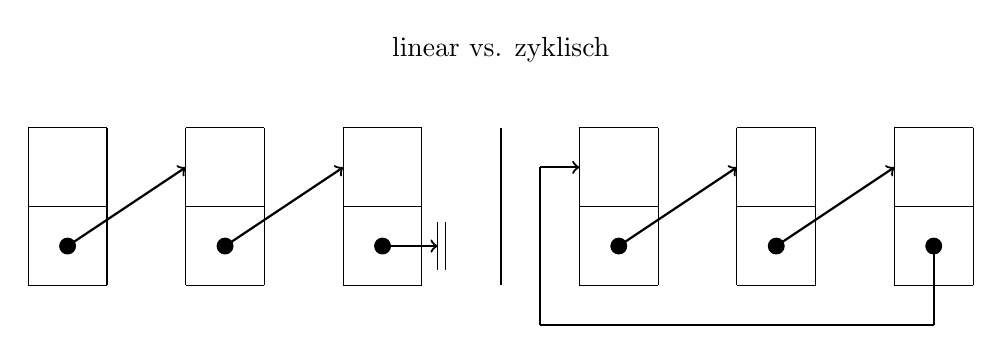
\begin{tikzpicture}
		\node at (0,0) (lz) {linear vs. zyklisch};
		\draw (-4,-1) -- (-3,-1);
		\draw (-4,-3) -- (-3,-3);
		\draw (-4,-1) -- (-4,-3);
		\draw (-3,-1) -- (-3,-3);
		\draw (-4,-2) -- (-3,-2);
		\draw[fill=black] (-3.5,-2.5) circle (0.1);
		\draw[->, thick] (-3.5,-2.5) -- (-2,-1.5);
		\draw (-6,-1) -- (-5,-1);
		\draw (-6,-3) -- (-5,-3);
		\draw (-6,-1) -- (-6,-3);
		\draw (-5,-1) -- (-5,-3);
		\draw (-6,-2) -- (-5,-2);
		\draw[fill=black] (-5.5,-2.5) circle (0.1);
		\draw[->, thick] (-5.5,-2.5) -- (-4,-1.5);
		\draw (-2,-1) -- (-1,-1);
		\draw (-2,-3) -- (-1,-3);
		\draw (-2,-1) -- (-2,-3);
		\draw (-1,-1) -- (-1,-3);
		\draw (-2,-2) -- (-1,-2);
		\draw[fill=black] (-1.5,-2.5) circle (0.1);
		\draw[->, thick] (-1.5,-2.5) -- (-0.8,-2.5);
		\draw (-0.8,-2.2) -- (-0.8,-2.8);
		\draw (-0.7,-2.2) -- (-0.7,-2.8);
		
		\draw[thick] (0,-1) -- (0,-3);
		
		\draw (4,-1) -- (3,-1);
		\draw (4,-3) -- (3,-3);
		\draw (4,-1) -- (4,-3);
		\draw (3,-1) -- (3,-3);
		\draw (4,-2) -- (3,-2);
		\draw[fill=black] (3.5,-2.5) circle (0.1);
		\draw[->, thick] (1.5,-2.5) -- (3,-1.5);
		\draw (6,-1) -- (5,-1);
		\draw (6,-3) -- (5,-3);
		\draw (6,-1) -- (6,-3);
		\draw (5,-1) -- (5,-3);
		\draw (6,-2) -- (5,-2);
		\draw[fill=black] (5.5,-2.5) circle (0.1);
		\draw[->, thick] (3.5,-2.5) -- (5,-1.5);
		\draw (2,-1) -- (1,-1);
		\draw (2,-3) -- (1,-3);
		\draw (2,-1) -- (2,-3);
		\draw (1,-1) -- (1,-3);
		\draw (2,-2) -- (1,-2);
		\draw[fill=black] (1.5,-2.5) circle (0.1);
		\draw[thick] (5.5,-2.5) -- (5.5,-3.5);
		\draw[thick] (5.5,-3.5) -- (0.5,-3.5);
		\draw[thick] (0.5,-3.5) -- (0.5,-1.5);
		\draw[->, thick] (0.5,-1.5) -- (1,-1.5);
	\end{tikzpicture}
\end{center}

\begin{center}
	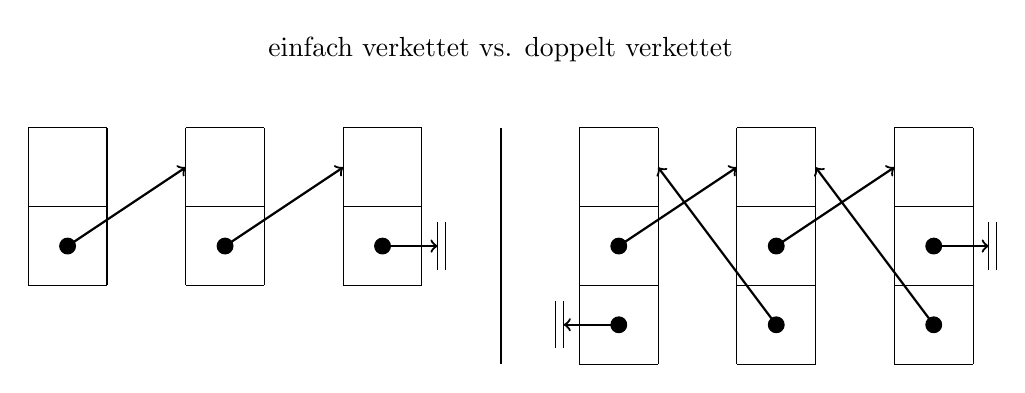
\begin{tikzpicture}
		\node at (0,0) (lz) {einfach verkettet vs. doppelt verkettet};
		\draw (-4,-1) -- (-3,-1);
		\draw (-4,-3) -- (-3,-3);
		\draw (-4,-1) -- (-4,-3);
		\draw (-3,-1) -- (-3,-3);
		\draw (-4,-2) -- (-3,-2);
		\draw[fill=black] (-3.5,-2.5) circle (0.1);
		\draw[->, thick] (-3.5,-2.5) -- (-2,-1.5);
		\draw (-6,-1) -- (-5,-1);
		\draw (-6,-3) -- (-5,-3);
		\draw (-6,-1) -- (-6,-3);
		\draw (-5,-1) -- (-5,-3);
		\draw (-6,-2) -- (-5,-2);
		\draw[fill=black] (-5.5,-2.5) circle (0.1);
		\draw[->, thick] (-5.5,-2.5) -- (-4,-1.5);
		\draw (-2,-1) -- (-1,-1);
		\draw (-2,-3) -- (-1,-3);
		\draw (-2,-1) -- (-2,-3);
		\draw (-1,-1) -- (-1,-3);
		\draw (-2,-2) -- (-1,-2);
		\draw[fill=black] (-1.5,-2.5) circle (0.1);
		\draw[->, thick] (-1.5,-2.5) -- (-0.8,-2.5);
		\draw (-0.8,-2.2) -- (-0.8,-2.8);
		\draw (-0.7,-2.2) -- (-0.7,-2.8);
		
		\draw[thick] (0,-1) -- (0,-4);
		
		\draw (4,-1) -- (3,-1);
		\draw (4,-3) -- (3,-3);
		\draw (4,-1) -- (4,-3);
		\draw (3,-1) -- (3,-3);
		\draw (4,-2) -- (3,-2);
		\draw[fill=black] (3.5,-2.5) circle (0.1);
		\draw[->, thick] (1.5,-2.5) -- (3,-1.5);
		\draw (4,-3) -- (4,-4);
		\draw (4,-4) -- (3,-4);
		\draw (3,-4) -- (3,-3);
		\draw[fill=black] (3.5,-3.5) circle (0.1);
		\draw[->, thick] (3.5,-3.5) -- (2,-1.5);
		\draw (6,-1) -- (5,-1);
		\draw (6,-3) -- (5,-3);
		\draw (6,-1) -- (6,-3);
		\draw (5,-1) -- (5,-3);
		\draw (6,-2) -- (5,-2);
		\draw[fill=black] (5.5,-2.5) circle (0.1);
		\draw[->, thick] (3.5,-2.5) -- (5,-1.5);
		\draw (2,-1) -- (1,-1);
		\draw (2,-3) -- (1,-3);
		\draw (2,-1) -- (2,-3);
		\draw (1,-1) -- (1,-3);
		\draw (2,-2) -- (1,-2);
		\draw (1,-3) -- (1,-4);
		\draw (1,-4) -- (2,-4);
		\draw (2,-4) -- (2,-3);
		\draw[fill=black] (1.5,-3.5) circle (0.1);
		\draw[->, thick] (1.5,-3.5) -- (0.8,-3.5);
		\draw (0.8,-3.2) -- (0.8,-3.8);
		\draw (0.7,-3.2) -- (0.7,-3.8);
		\draw[fill=black] (1.5,-2.5) circle (0.1);
		\draw[->, thick] (5.5,-2.5) -- (6.2,-2.5);
		\draw (6.2,-2.2) -- (6.2,-2.8);
		\draw (6.3,-2.2) -- (6.3,-2.8);
		\draw (6,-3) -- (6,-4);
		\draw (5,-4) -- (6,-4);
		\draw (5,-4) -- (5,-3);
		\draw[fill=black] (5.5,-3.5) circle (0.1);
		\draw[->, thick] (5.5,-3.5) -- (4,-1.5);
	\end{tikzpicture}
\end{center}

Eine Liste hat immer gewisse Einfüge- und Löschoperationen. Wenn diese an beiden Enden der Liste notwendig sind, spricht man von einer \begriff{Deque} = double-ended-queue.

\subsection{Grundoperationen auf einer Liste}

\begin{longtable}{p{0.25\textwidth}|p{0.4\textwidth}|p{0.25\textwidth}}
	\texttt{init(L)} & Initalisierung der Liste, Anfangszustand "'leer"' & \\
	\hline
	\texttt{empty(L)} & als Abfragefunktion $\to$ \texttt{.true.} falls \texttt{L} leer, sonst \texttt{.false.} & \\
	\hline
	\texttt{access\_head(L,e)} & als Subroutine, gibt in \texttt{e} den Wert des head-Elements & head = Beginn einer Liste \\
	\hline
	\texttt{val\_head(L)} & als Funktion $\to$ Ergebnis ist Inhalt des head-Elements & \\
	\hline
	\texttt{access\_tail(L,e)} & als Subroutine, gibt in \texttt{e} den Wert des tail-Elements & tail = Ende einer Liste \\
	\hline
	\texttt{val\_tail(L)} & als Funktion $\to$ Ergebnis ist Inhalt des tail-Elements & \\
	\hline
	\texttt{val\_elem(L,p)} & liefert Inhalt des durch \texttt{p} referenzierten Elements & \\
	\hline
	\multicolumn{3}{p{\textwidth}}{\cellcolor{lightgray}\textbf{insert}} \\
	\hline
	\texttt{insert\_head(L,e)} & Einfügen des Elements \texttt{e} am Anfang der Liste \texttt{L} & anderer Name: \texttt{push} \\
	\hline
	\texttt{insert\_tail(L,e)} & Einfügen des Elements \texttt{e} am Ende der Liste \texttt{L} & anderer Name: \texttt{inject} \\
	\hline
	\texttt{insert\_after(L,p,e)} & Einfügen des Elements \texttt{e} nach dem von \texttt{p} referenzierten Element & \\
	\hline
	\texttt{insert\_before(L,p,e)} & Einfügen des Elements \texttt{e} vor dem von \texttt{p} referenzierten Element & \\
	\hline
	\multicolumn{3}{p{\textwidth}}{\cellcolor{lightgray}\textbf{delete}} \\
	\hline
	\texttt{del\_head(L,e)} & Löschen des Elements \texttt{e} am Anfang der Liste \texttt{L} & anderer Name: \texttt{pop} \\
	\hline
	\texttt{del\_tail(L,e)} & Löschen des Elements \texttt{e} am Ende der Liste \texttt{L} & anderer Name: \texttt{eject} \\
	\hline
	\texttt{del\_after(L,p,e)} & Löschen des Elements \texttt{e} nach dem von \texttt{p} referenzierten Element & \\
	\hline
	\texttt{del\_elem(L,p,e)} & Löschen eines Elements \texttt{e}, welches von \texttt{p} referenziert wird & \\
	\hline
	\multicolumn{3}{p{\textwidth}}{\cellcolor{lightgray}\textbf{Traversieren (Durchlaufen aller Elemente) der Liste \texttt{L} und Ausführen einer Task \texttt{T} auf jedem Element}} \\
	\hline
	\texttt{trav\_forward(L,T[,p])} & vorwärts, optional ab dem von \texttt{p} referenzierten Element \\
	\hline
	\texttt{trav\_backward(L,T[,p])} & rückwärts, optional ab dem von \texttt{p} referenzierten Element \\
	\hline
	\multicolumn{3}{p{\textwidth}}{\cellcolor{lightgray}\textbf{Suchen eines Elements mit dem Inhalt \texttt{e}}} \\
	\hline
	\texttt{find\_forward(L,e[,p])} & vorwärts, optional ab dem von \texttt{p} referenzierten Element \\
	\hline
	\texttt{find\_backward(L,e[,p])} & rückwärts, optional ab dem von \texttt{p} referenzierten Element \\
\end{longtable}

\subsection{Grundoperationen auf einer Deque}

Der einfachste Fall ist der einer linearen, nicht zyklischen, einfach verketteten, endogenen Liste mit \texttt{s} als head-Pointer.

\subsubsection*{\texttt{push(s,elem)}}

\begin{center}
	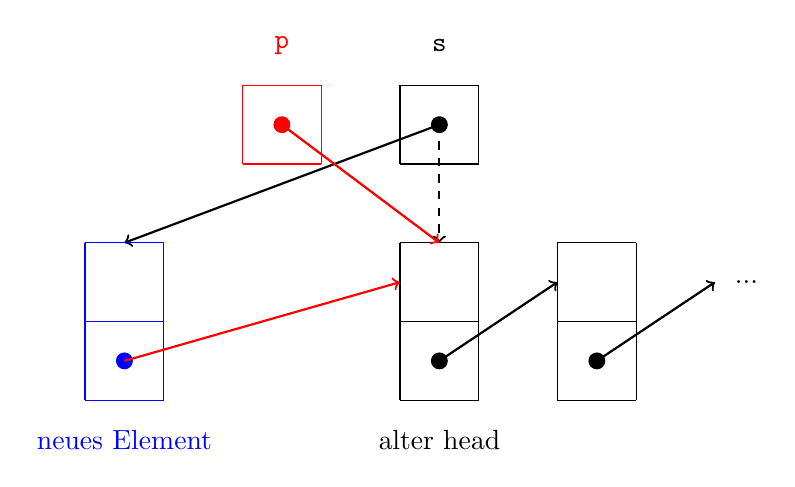
\begin{tikzpicture}
	\draw (0,-1) -- (1,-1);
	\draw (0,-2) -- (1,-2);
	\draw (0,-1) -- (0,-2);
	\draw (1,-1) -- (1,-2);
	\draw[fill=black] (0.5,-1.5) circle (0.1);
	\draw[->, thick, dashed] (0.5,-1.5) -- (0.5,-3);
	\draw[->, thick] (0.5,-1.5) -- (-3.5,-3);
	\node at (0.5,-0.5) (s) {\texttt{s}};
	
	\draw (0,-3) -- (0,-5);
	\draw (0,-3) -- (1,-3);
	\draw (1,-3) -- (1,-5);
	\draw (0,-5) -- (1,-5);
	\draw (0,-4) -- (1,-4);
	\draw[fill=black] (0.5,-4.5) circle (0.1);
	\draw[->, thick] (0.5,-4.5) -- (2,-3.5);
	\node at (0.5,-5.5) (alt) {alter head};
	
	\draw (2,-3) -- (2,-5);
	\draw (2,-3) -- (3,-3);
	\draw (3,-3) -- (3,-5);
	\draw (2,-5) -- (3,-5);
	\draw (2,-4) -- (3,-4);
	\draw[fill=black] (2.5,-4.5) circle (0.1);
	\draw[->, thick] (2.5,-4.5) -- (4,-3.5);
	\node at (4.4,-3.5) (n) {...};
	
	\draw[red] (-2,-1) -- (-1,-1);
	\draw[red] (-2,-2) -- (-1,-2);
	\draw[red] (-2,-1) -- (-2,-2);
	\draw[red] (-1,-1) -- (-1,-2);
	\draw[fill=red, red] (-1.5,-1.5) circle (0.1);
	\draw[->, thick, red] (-1.5,-1.5) -- (0.5,-3);
	\node[red] at (-1.5,-0.5) (s) {\texttt{p}};
	
	\draw[blue] (-4,-3) -- (-3,-3);
	\draw[blue] (-4,-3) -- (-4,-5);
	\draw[blue] (-3,-3) -- (-3,-5);
	\draw[blue] (-4,-4) -- (-3,-4);
	\draw[blue] (-4,-5) -- (-3,-5);
	\draw[fill=blue, blue] (-3.5,-4.5) circle (0.1);
	\draw[->, thick, red] (-3.5,-4.5) -- (0,-3.5);
	\node[blue] at (-3.5,-5.5) (neu) {neues Element};
	\end{tikzpicture}
\end{center}

Zuerst haben wir die schwarze Liste mit \texttt{s} als heap-Pointer. Für spätere Verwendung setzen wir noch den Nachfolger eines \textcolor{red}{\texttt{p}}-Pointer auf den head. Jetzt wird das \textcolor{blue}{neue Element} eingefügt und der \texttt{s}-Pointer zeigt auf den neuen head. Der Nachfolger des neuen head muss nun noch auf \textcolor{red}{\texttt{p}} zeigen, was ja auf den alten head zeigt. Schon ist das \textcolor{blue}{neue Element} eingebunden.

\subsubsection*{\texttt{pop(s,elem)}}

\begin{center}
	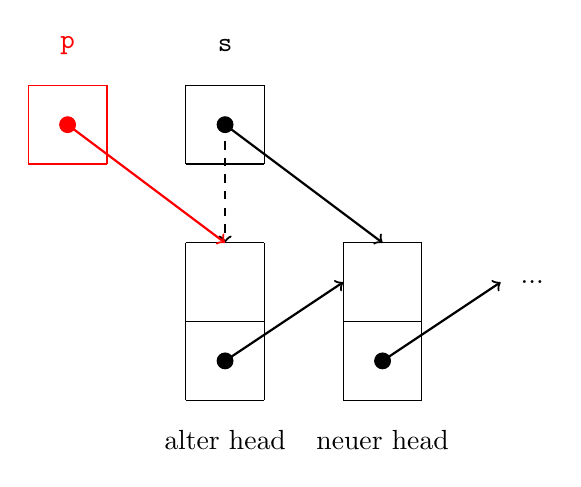
\begin{tikzpicture}
	\draw (0,-1) -- (1,-1);
	\draw (0,-2) -- (1,-2);
	\draw (0,-1) -- (0,-2);
	\draw (1,-1) -- (1,-2);
	\draw[fill=black] (0.5,-1.5) circle (0.1);
	\draw[->, thick, dashed] (0.5,-1.5) -- (0.5,-3);
	\draw[->, thick] (0.5,-1.5) -- (2.5,-3);
	\node at (0.5,-0.5) (s) {\texttt{s}};
	
	\draw (0,-3) -- (0,-5);
	\draw (0,-3) -- (1,-3);
	\draw (1,-3) -- (1,-5);
	\draw (0,-5) -- (1,-5);
	\draw (0,-4) -- (1,-4);
	\draw[fill=black] (0.5,-4.5) circle (0.1);
	\draw[->, thick] (0.5,-4.5) -- (2,-3.5);
	\node at (0.5,-5.5) (alt) {alter head};
	
	\draw (2,-3) -- (2,-5);
	\draw (2,-3) -- (3,-3);
	\draw (3,-3) -- (3,-5);
	\draw (2,-5) -- (3,-5);
	\draw (2,-4) -- (3,-4);
	\draw[fill=black] (2.5,-4.5) circle (0.1);
	\draw[->, thick] (2.5,-4.5) -- (4,-3.5);
	\node at (2.5,-5.5) (neu) {neuer head};
	\node at (4.4,-3.5) (n) {...};
	
	\draw[red] (-2,-1) -- (-1,-1);
	\draw[red] (-2,-2) -- (-1,-2);
	\draw[red] (-2,-1) -- (-2,-2);
	\draw[red] (-1,-1) -- (-1,-2);
	\draw[fill=red, red] (-1.5,-1.5) circle (0.1);
	\draw[->, thick, red] (-1.5,-1.5) -- (0.5,-3);
	\node[red] at (-1.5,-0.5) (s) {\texttt{p}};
	\end{tikzpicture}
\end{center}

Wir haben wieder die schwarze Liste mit \texttt{s}-Pointer. Um auf den alten head zugreifen zu können, benutzen wir wieder den Hilfspointer \textcolor{red}{\texttt{p}}. Den \texttt{s}-Pointer setzen wir dann auf den Nachfolger des alten heads.

\subsubsection*{\texttt{inject(t,elem)}}

Der Nachfolger des alten tails zeigt nun auf das neue Element. Dann muss nur noch der tail-Pointer angepasst werden und der Nachfolger des neuen tails muss mit \texttt{nullify} auf Null gesetzt werden.

\subsubsection*{\texttt{eject(t,elem)}}

Hier bekommen wir ein Problem! Nicht das es nicht möglich wäre das letzte Element zu löschen, aber der Vorgänger des tail-Elements kann nur gefunden werden, indem man die ganze Liste durchläuft. Das heißt die Laufzeitkomplexität dieser Operation beträgt $T(n)=\mathcal{O}(n)$. Die Dauer dieser Operation ist also von der Listenlänge abhängig!